\ifdefined\iscombined
	\lecturetitle{Rotational Mechanical Systems}
\else
\documentclass{article}
\usepackage{xparse}
\usepackage{changepage}
\usepackage{listings}
\usepackage{amsthm}
\usepackage{comment}
\usepackage{amsmath}
\usepackage{braket}
\usepackage{amsfonts}
\usepackage{sectsty}
\usepackage{hyperref}
\usepackage{fancyhdr}
\usepackage[top=1in,bottom=1in,left=1in,right=1in]{geometry}
\usepackage{float}
\usepackage{graphicx}
\usepackage{mathtools}
\usepackage{tikz}
\usetikzlibrary{arrows,calc,patterns,decorations.pathmorphing,decorations.markings,shapes.geometric}
\usepackage{circuitikz}

\date{
	\vspace{-.75em}
	{\large \today}
}

\title{
	\vspace*{-1.5em}
	{\Huge Lecture 11} \\
	\vspace{-1em}
	\rule{\textwidth/4}{.01em} \\
	\vspace{-.25em}
	{\Large Rotational Mechanical Systems}
	\vspace{-.75em}
}

\author{
	{\large Matthew Farah}
}

\hypersetup{
	colorlinks=true,
	linkcolor=blue,
	filecolor=magenta,
	urlcolor=blue,
	citecolor=blue,
	anchorcolor=blue
}

\fancyhead{}
\fancyhead[L]{\today}
\fancyhead[R]{Lecture 11 - Rotational Mechanical Systems}

\setlength{\parindent}{0cm}

\newcounter{example}
\renewcommand{\theexample}{\arabic{example}}

\newenvironment{example}[1][]{
	\refstepcounter{example}
	\begin{adjustwidth}{1.5em}{}
	\vspace{1em}
	\noindent\textbf{\ifx&#1&Example \theexample:\else Example \theexample \ (#1):\fi}
	\ignorespaces
}{
	\vspace{.5em}
	\end{adjustwidth}
}

\newenvironment{solution}{
	\vspace{.5em}
	\par
	\begin{adjustwidth}{1.5em}{}
	\textbf{{Solution:}}
	\par
	\vspace{.5em}
}{
	\vspace{1em}
	\end{adjustwidth}
}

\newcounter{subexample}
\renewcommand{\thesubexample}{\alph{subexample}}

\newenvironment{subexample}{
	\setcounter{step}{0}
	\refstepcounter{subexample}
	\vspace{1em}\par\noindent
	\begin{adjustwidth}{1.5em}{}
	\noindent\textbf{(\thesubexample)}
	\ignorespaces
}{
	\par
	\vspace{1em}
	\end{adjustwidth}
}

\renewenvironment{proof}{
	\vspace{.5em}\par\noindent
	\begin{adjustwidth}{1.5em}{}
	\emph{Proof:}\par\vspace{1em}
	\setlength{\parindent}{0cm}
}{
	\end{adjustwidth}
}

\newtheorem{theorem}{Theorem}

\renewenvironment{theorem}[1][]{
	\refstepcounter{theorem}
	\vspace{1em}\par\noindent
	\begin{adjustwidth}{1.5em}{}
	\noindent\textbf{\ifx&#1&Theorem \thetheorem:\else Theorem \thetheorem \ (#1):\fi}
	\ignorespaces
}{
	\vspace{.5em}
	\end{adjustwidth}
}

\newtheorem{lemma}{Lemma}

\renewenvironment{lemma}[1][]{
	\refstepcounter{lemma}
	\vspace{1em}\par\noindent
	\begin{adjustwidth}{1.5em}{}
	\noindent\textbf{\ifx&#1&Lemma \thelemma:\else Lemma \thelemma \ (#1):\fi}
	\ignorespaces
}{
	\vspace{.5em}
	\end{adjustwidth}
}

\makeatother
\makeatletter

\newcounter{step}
\renewcommand{\thestep}{\Roman{step}}

\newenvironment{step}{
	\refstepcounter{step}
	\vspace{1em}\par\noindent
	\ignorespaces\noindent\textbf{(\thestep)}
	\ignorespaces
}{
	\par
	\vspace{1em}
}

\sectionfont{\fontsize{12}{12}\bfseries}
\subsectionfont{\fontsize{10}{12}\normalfont}
\subsubsectionfont{\fontsize{10}{12}\normalfont}

\begin{document}

\maketitle
\pagestyle{fancy}

\fi

\begin{itemize}
	\item The degrees of freedom of a rotational system is given by the number of linearly independent rotations in the system.
	\begin{itemize}
		\item Two inertias have linearly independent rotations if holding one in place still allows for the other to rotate.
		\item The degrees of freedom of a rotational system can be more tricky to determine than of translational systems.
	\end{itemize}

	\item Impedances in rotational systems work as follows:
	\begin{itemize}
		\item A moment of inertia $J$ imparts an impedance of $Js^2$ on a rotating body.
		\item A viscous damper with a damping constant $D$ imparts an impedance of $Ds$ on a rotating body.
		\item A spring with a spring constant $K$ imparts an impedance of $K$ on a rotating body.
	\end{itemize}
	\item The transfer function of rotational systems describes the ratio between a body's rotation and an applied torque:
\end{itemize}

\begin{align*}
	G(s) &= \frac{\Theta_i(s)}{T(s)}
\end{align*}

\begin{example}
	Find the transfer function $G(s) = \frac{\Theta_2(s)}{T(s)}$ for the following system:

	\vspace{1em}

	\begin{figure}[H]
		\centering
		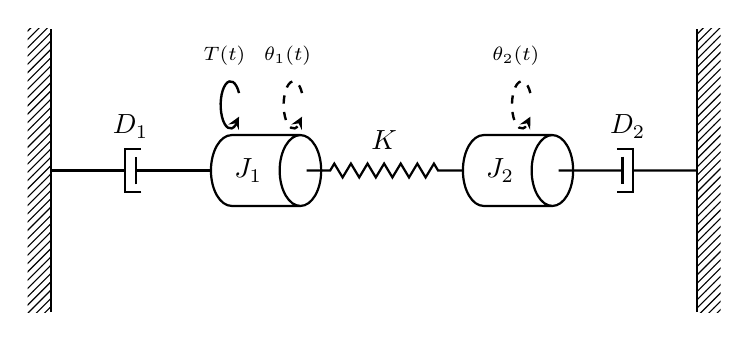
\begin{tikzpicture}[>=latex]
			\tikzstyle{spring}=[thick,decorate,decoration={zigzag,pre length=0.3cm,post length=0.3cm,segment length=6}]
			\tikzstyle{damper}=[thick,decoration={markings,
				mark connection node=dmp,
				mark=at position 0.5 with
				{
					\node (dmp) [thick,inner sep=0pt,transform shape,rotate=-90,minimum width=15pt,minimum height=3pt,draw=none] {};
					\draw [thick] ($(dmp.north east)+(2pt,0)$) -- (dmp.south east) -- (dmp.south west) -- ($(dmp.north west)+(2pt,0)$);
					\draw [thick] ($(dmp.north)+(0,-5pt)$) -- ($(dmp.north)+(0,5pt)$);
				}
			}, decorate]

			\newcommand{\AxisRotator}[1][rotate=0]{
				\tikz [x=0.25cm,y=0.60cm,line width=.2ex,-stealth,#1] \draw (0,0) arc (-150:150:1 and 1);
			}

			\fill [pattern=north east lines] (0,-1.8) rectangle (0.3,1.8);
			\draw [thick] (0.3,-1.8) -- (0.3,1.8);

			\node (J1) [thick, cylinder, draw, minimum width=0.9cm, minimum height=1.4cm] at (2.8,0) {$J_1$};

			\draw [damper] (0.3,0) -- (J1.west) node[midway, above=8pt, fill=white] {$D_1$};

			\node (J2) [thick, cylinder, draw, fill=white, minimum width=0.9cm, minimum height=1.4cm] at (6,0) {$J_2$};

			\draw [spring] ($(J1.east) + (-0.2, 0)$) -- (J2.west) node[midway, above=4pt, fill=white] {$K$};

			\draw [damper] (8.5,0) -- ($(J2.east) + (-0.2, 0)$)   node[midway, above=8pt, fill=white] {$D_2$};

			\draw [thick] (8.5,-1.8) -- (8.5,1.8);
			\fill [pattern=north east lines] (8.5,-1.8) rectangle (8.8,1.8);

			\draw ($(J1.center) + (-0.3, 0)$)  node[above=10pt, label={[label distance = -3pt, font=\scriptsize]above:{$T(t)$}}] {\AxisRotator[rotate = 180, scale=.5]};
			\draw ($(J1.center) + (0.5, 0)$)  node[above=10pt, label={[label distance = -3pt, font=\scriptsize]above:{$\theta_1(t)$}}] {\AxisRotator[rotate = 180, dashed, scale=.5]};
			\draw ($(J2.center) + (0.2, 0)$)  node[above=10pt, label={[label distance = -3pt, font=\scriptsize]above:{$\theta_2(t)$}}] {\AxisRotator[rotate = 180, dashed, scale=.5]};
		\end{tikzpicture}
	\end{figure}

	\vspace{1em}
\end{example}

\begin{solution}
	First, it is important to notice that the given system has two degrees of freedom. \\

	Analogously to translational systems, we can construct FBDs for each rotating body by leveraging Newton's second law of motion and the superposition principle. In the interest of not beating a dead horse, we can see the following FBDs accurately represent the given system:

	\vspace{1em}

	\begin{figure}[H]
		\centering
		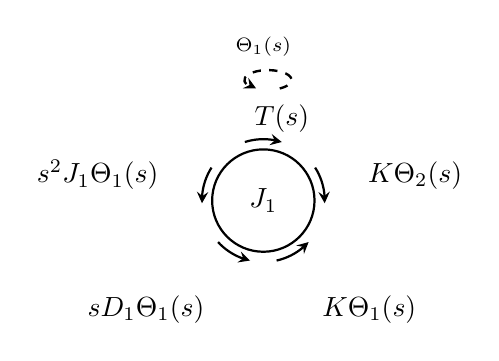
\begin{tikzpicture}[>=stealth]
			\newcommand{\AxisRotator}[1][rotate=0]{
				\tikz [x=0.25cm,y=0.60cm,line width=.2ex,-stealth,#1] \draw (0,0) arc (-150:150:1 and 1);
			}

			\node (J1) [thick, circle, draw, minimum size=1.3cm] at (0,0) {$J_1$};

			\draw ($(J1.north) + (0,0.55)$) node[above=2pt, label={[label distance = -3pt, font=\scriptsize]above:{$\Theta_1(s)$}}] {\AxisRotator[rotate = 90, dashed, scale=.5]};

			\def\R{0.78}
			\def\LR{1.25}
			\def\ArcSpan{35}

			\draw[<-, thick] ($(J1.center) + ({90 - \ArcSpan/2}:\R)$) arc ({90 - \ArcSpan/2}:{90 + \ArcSpan/2}:\R);
			\node[above right] at ($(J1.center) + ({90 + \ArcSpan/2}:\R)$) {$T(s)$};

			\draw[<-, thick] ($(J1.center) + ({15 - \ArcSpan/2}:\R)$) arc ({15 - \ArcSpan/2}:{15 + \ArcSpan/2}:\R);
			\node[right] at ($(J1.center) + (15:\LR)$) {$K \Theta_2(s)$};

			\draw[->, thick] ($(J1.center) + ({-60 - \ArcSpan/2}:\R)$) arc ({-60 - \ArcSpan/2}:{-60 + \ArcSpan/2}:\R);
			\node[below right] at ($(J1.center) + (-60:\LR)$) {$K \Theta_1(s)$};

			\draw[->, thick] ($(J1.center) + ({-120 - \ArcSpan/2}:\R)$) arc ({-120 - \ArcSpan/2}:{-120 + \ArcSpan/2}:\R);
			\node[below left] at ($(J1.center) + (-120:\LR)$) {$s D_1 \Theta_1(s)$};

			\draw[->, thick] ($(J1.center) + ({165 - \ArcSpan/2}:\R)$) arc ({165 - \ArcSpan/2}:{165 + \ArcSpan/2}:\R);
			\node[left] at ($(J1.center) + (165:\LR)$) {$s^2 J_1 \Theta_1(s)$};
		\end{tikzpicture}
		\hspace{3em}
		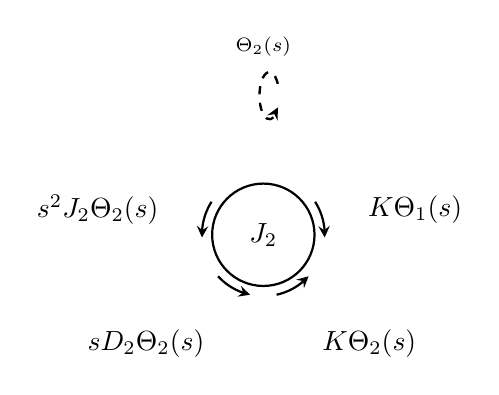
\begin{tikzpicture}[>=stealth]
			\newcommand{\AxisRotator}[1][rotate=0]{
				\tikz [x=0.25cm,y=0.60cm,line width=.2ex,-stealth,#1] \draw (0,0) arc (-150:150:1 and 1);
			}

			\node (J2) [thick, circle, draw, minimum size=1.3cm] at (0,0) {$J_2$};

			\draw ($(J2.north) + (0,0.55)$) node[above=2pt, label={[label distance = -3pt, font=\scriptsize]above:{$\Theta_2(s)$}}] {\AxisRotator[rotate = 180, dashed, scale=.5]};

			\def\R{0.78}
			\def\LR{1.25}
			\def\ArcSpan{35}

			\draw[<-, thick] ($(J2.center) + ({15 - \ArcSpan/2}:\R)$) arc ({15 - \ArcSpan/2}:{15 + \ArcSpan/2}:\R);
			\node[right] at ($(J2.center) + (15:\LR)$) {$K \Theta_1(s)$};

			\draw[->, thick] ($(J2.center) + ({-60 - \ArcSpan/2}:\R)$) arc ({-60 - \ArcSpan/2}:{-60 + \ArcSpan/2}:\R);
			\node[below right] at ($(J2.center) + (-60:\LR)$) {$K \Theta_2(s)$};

			\draw[->, thick] ($(J2.center) + ({-120 - \ArcSpan/2}:\R)$) arc ({-120 - \ArcSpan/2}:{-120 + \ArcSpan/2}:\R);
			\node[below left] at ($(J2.center) + (-120:\LR)$) {$s D_2 \Theta_2(s)$};

			\draw[->, thick] ($(J2.center) + ({165 - \ArcSpan/2}:\R)$) arc ({165 - \ArcSpan/2}:{165 + \ArcSpan/2}:\R);
			\node[left] at ($(J2.center) + (165:\LR)$) {$s^2 J_2 \Theta_2(s)$};
		\end{tikzpicture}
	\end{figure}

	\vspace{1em}

	By Newton's third law of motion, summing the torques on $J_1$ gives:

	\begin{equation*}
		\begin{array}{lrl}
			& s^2 J_1 \Theta_1(s) + s D_1 \Theta_1(s) + K \Theta_1(s) =& T(s) + K \Theta_2(s) \\
			\implies & s^2 J_1 \Theta_1(s) + s D_1 \Theta_1(s) + K \Theta_1(s) - K \Theta_2(s) =& T(s) \\
			\implies & (s^2 J_1 + s D_1 + K) \Theta_1(s) - K \Theta_2(s) =& T(s) \quad \ldots (1)
		\end{array}
	\end{equation*} \\

	And similarly for $J_2$:

	\begin{equation*}
		\begin{array}{lrl}
			& s^2 J_2 \Theta_2(s) + s D_2 \Theta_2(s) + K \Theta_2(s) =& K \Theta_1(s) \\
			\implies & -K \Theta_1(s) + s^2 J_2 \Theta_2(s) + s D_2 \Theta_2(s) + K \Theta_2(s) =& 0 \\
			\implies & -K \Theta_1(s) + (s^2 J_2 + s D_2 + K) \Theta_2(s) =& 0 \quad \ldots (2)
		\end{array}
	\end{equation*} \\

	Putting equations $(1)$ and $(2)$ into matrix form, we see that:

	\begin{align*}
		\begin{bmatrix} J_1 s^2 + D_1 s + K & -K \\\\ -K & J_2 s^2 + D_2 s + K \end{bmatrix} \begin{bmatrix} \Theta_1(s) \\\\ \Theta_2(s) \end{bmatrix} &= \begin{bmatrix} T(s) \\\\ 0 \end{bmatrix} \\
	\end{align*}

	And so, letting $A$ be the left-most matrix above and $A_2$ be the result of replacing the second column of $A$ with $\begin{bmatrix} T(s) \\\\ 0 \end{bmatrix}$:

	\begin{align*}
		A_2 &= \begin{bmatrix} J_1 s^2 + D_1 s + K & T(s) \\\\ -K & 0 \end{bmatrix} \\\\
	\end{align*}

	We can compute:

	\begin{align*}
		\det(A) &= (J_1 s^2 + D_1 s + K)(J_2 s^2 + D_2 s + K) - (-K)(-K) \\
			&= J_1 J_2 s^4 + (J_1 D_2 + J_2 D_1) s^3 + (J_1 K + D_1 D_2 + J_2 K) s^2 + (D_1 + D_2) K s \\
	\end{align*}

	And:

	\begin{align*}
		\det(A_2) &= (J_1 s^2 + D_1 s + K)(0) - (T(s))(-K) \\
			&= K T(s) \\
	\end{align*}

	Hence by Cramer's rule:

	\begin{align*}
		\Theta_2(s) &= \frac{\det(A_2)}{\det(A)} = \frac{K T(s)}{J_1 J_2 s^4 + (J_1 D_2 + J_2 D_1) s^3 + (J_1 K + D_1 D_2 + J_2 K) s^2 + (D_1 + D_2) K s} \\
	\end{align*}

	And thus we can conclude that:

	\begin{align*}
		G(s) &= \frac{\Theta_2(s)}{T(s)} = \frac{K}{J_1 J_2 s^4 + (J_1 D_2 + J_2 D_1) s^3 + (J_1 K + D_1 D_2 + J_2 K) s^2 + (D_1 + D_2) K s} \\
	\end{align*}
\end{solution}

\begin{example}
	Determine how many degrees of freedom the following system has:

	\vspace{1em}

	\begin{figure}[H]
		\centering
		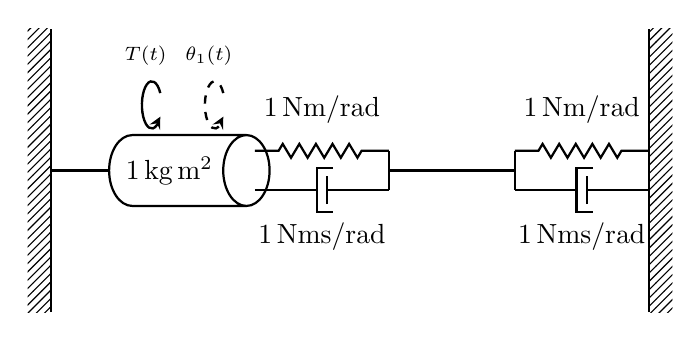
\begin{tikzpicture}[>=latex]
			\tikzstyle{spring}=[thick,decorate,decoration={zigzag,pre length=0.3cm,post length=0.3cm,segment length=6}]
			\tikzstyle{damper}=[thick,decoration={markings,
				mark connection node=dmp,
				mark=at position 0.5 with
				{
					\node (dmp) [thick,inner sep=0pt,transform shape,rotate=-90,minimum width=15pt,minimum height=3pt,draw=none] {};
					\draw [thick] ($(dmp.north east)+(2pt,0)$) -- (dmp.south east) -- (dmp.south west) -- ($(dmp.north west)+(2pt,0)$);
					\draw [thick] ($(dmp.north)+(0,-5pt)$) -- ($(dmp.north)+(0,5pt)$);
				}
			}, decorate]

			\newcommand{\AxisRotator}[1][rotate=0]{
				\tikz [x=0.25cm,y=0.60cm,line width=.2ex,-stealth,#1] \draw (0,0) arc (-150:150:1 and 1);
			}

			\fill [pattern=north east lines] (0,-1.8) rectangle (0.3,1.8);
			\draw [thick] (0.3,-1.8) -- (0.3,1.8);

			\node (J1) [thick, cylinder, draw, minimum width=0.9cm, minimum height=1.4cm] at (1.8,0) {$1\,\text{kg}\,\text{m}^2$};

			\draw [thick] (0.3,0) -- (J1.west);

			\draw [spring] ($(J1.east) + (-0.2, 0.25)$) -- ($(J1.east) + (1.5, 0.25)$) node[midway, above=6pt, fill=white] {$1\,\text{Nm/rad}$};
			\draw [damper] ($(J1.east) + (-0.2, -0.25)$) -- ($(J1.east) + (1.5, -0.25)$) node[midway, below=8pt, fill=white] {$1\,\text{Nms/rad}$};
			\draw [thick] ($(J1.east) + (1.5, 0.25)$) -- ($(J1.east) + (1.5, -0.25)$);

			\draw [thick] ($(J1.east) + (1.5, 0)$) -- ($(J1.east) + (3.1, 0)$);

			\draw [thick] ($(J1.east) + (3.1, 0.25)$) -- ($(J1.east) + (3.1, -0.25)$);

			\draw [spring] ($(J1.east) + (3.1, 0.25)$) -- ($(J1.east) + (4.8, 0.25)$) node[midway, above=6pt, fill=white] {$1\,\text{Nm/rad}$};
			\draw [damper] ($(J1.east) + (3.1, -0.25)$) -- ($(J1.east) + (4.8, -0.25)$) node[midway, below=8pt, fill=white] {$1\,\text{Nms/rad}$};

			\draw [thick] ($(J1.east) + (4.8, -1.8)$) -- ($(J1.east) + (4.8, 1.8)$);
			\fill [pattern=north east lines] ($(J1.east) + (4.8, -1.8)$) rectangle ($(J1.east) + (5.1, 1.8)$);

			\draw ($(J1.center) + (-0.3, 0)$) node[above=10pt, label={[label distance = -3pt, font=\scriptsize]above:{$T(t)$}}] {\AxisRotator[rotate = 180, scale=.5]};
			\draw ($(J1.center) + (0.5, 0)$) node[above=10pt, label={[label distance = -3pt, font=\scriptsize]above:{$\theta_1(t)$}}] {\AxisRotator[rotate = 180, dashed, scale=.5]};
		\end{tikzpicture}
	\end{figure}

	\vspace{1em}
\end{example}

\begin{solution}
	Unintuitively, this system actually has two degrees of freedom, despite only having a single body with an inertia! \\

	It is clear that the body with an inertia of $1\,\text{kg}\,\text{m}^2$ constitutes one degree of freedom for the system. To see the other, consider locking that body in place such that it cannot rotate. \\

	Because of the way the rods between the springs and viscous dampers connect, even when holding the body still, we could apply a torque on the rod connecting the springs and viscous dampers to induce a rotation on the system. This gives an extra degree of freedom! \\

	To see this more clearly, we could equivalently redraw the system like so:

	\vspace{1em}

	\begin{figure}[H]
		\centering
		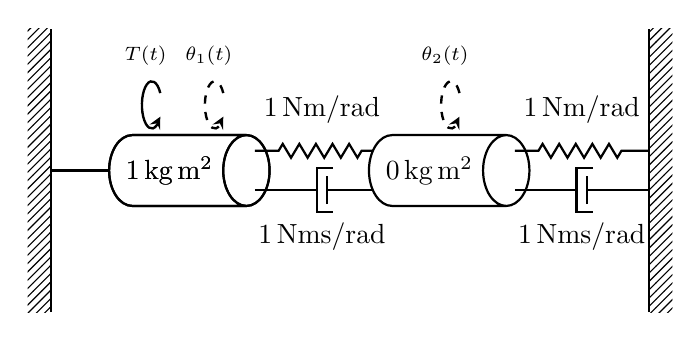
\begin{tikzpicture}[>=latex]
			\tikzstyle{spring}=[thick,decorate,decoration={zigzag,pre length=0.3cm,post length=0.3cm,segment length=6}]
			\tikzstyle{damper}=[thick,decoration={markings,
				mark connection node=dmp,
				mark=at position 0.5 with
				{
					\node (dmp) [thick,inner sep=0pt,transform shape,rotate=-90,minimum width=15pt,minimum height=3pt,draw=none] {};
					\draw [thick] ($(dmp.north east)+(2pt,0)$) -- (dmp.south east) -- (dmp.south west) -- ($(dmp.north west)+(2pt,0)$);
					\draw [thick] ($(dmp.north)+(0,-5pt)$) -- ($(dmp.north)+(0,5pt)$);
				}
			}, decorate]

			\newcommand{\AxisRotator}[1][rotate=0]{
				\tikz [x=0.25cm,y=0.60cm,line width=.2ex,-stealth,#1] \draw (0,0) arc (-150:150:1 and 1);
			}

			\fill [pattern=north east lines] (0,-1.8) rectangle (0.3,1.8);
			\draw [thick] (0.3,-1.8) -- (0.3,1.8);

			\node (J1) [thick, cylinder, draw, minimum width=0.9cm, minimum height=1.4cm] at (1.8,0) {$1\,\text{kg}\,\text{m}^2$};

			\draw [thick] (0.3,0) -- (J1.west);

			\draw [spring] ($(J1.east) + (-0.2, 0.25)$) -- ($(J1.east) + (1.5, 0.25)$) node[midway, above=6pt, fill=white] {$1\,\text{Nm/rad}$};
			\draw [damper] ($(J1.east) + (-0.2, -0.25)$) -- ($(J1.east) + (1.5, -0.25)$) node[midway, below=8pt, fill=white] {$1\,\text{Nms/rad}$};

			\node (J2) [thick, cylinder, draw, fill=white, minimum width=0.9cm, minimum height=1.4cm] at (5.1,0) {$0\,\text{kg}\,\text{m}^2$};

			\draw [spring] ($(J1.east) + (3.1, 0.25)$) -- ($(J1.east) + (4.8, 0.25)$) node[midway, above=6pt, fill=white] {$1\,\text{Nm/rad}$};
			\draw [damper] ($(J1.east) + (3.1, -0.25)$) -- ($(J1.east) + (4.8, -0.25)$) node[midway, below=8pt, fill=white] {$1\,\text{Nms/rad}$};

			\draw [thick] ($(J1.east) + (4.8, -1.8)$) -- ($(J1.east) + (4.8, 1.8)$);
			\fill [pattern=north east lines] ($(J1.east) + (4.8, -1.8)$) rectangle ($(J1.east) + (5.1, 1.8)$);

			\draw ($(J1.center) + (-0.3, 0)$) node[above=10pt, label={[label distance = -3pt, font=\scriptsize]above:{$T(t)$}}] {\AxisRotator[rotate = 180, scale=.5]};
			\draw ($(J1.center) + (0.5, 0)$) node[above=10pt, label={[label distance = -3pt, font=\scriptsize]above:{$\theta_1(t)$}}] {\AxisRotator[rotate = 180, dashed, scale=.5]};

			\node (J1) [thick, cylinder, draw, minimum width=0.9cm, minimum height=1.4cm] at (1.8,0) {$1\,\text{kg}\,\text{m}^2$};

			\draw [thick] (0.3,0) -- (J1.west);

			\draw ($(J2.center) + (0.2, 0)$) node[above=10pt, label={[label distance = -3pt, font=\scriptsize]above:{$\theta_2(t)$}}] {\AxisRotator[rotate = 180, dashed, scale=.5]};
		\end{tikzpicture}
	\end{figure}

	\vspace{1em}

	And since this equivalent system has two degrees of freedom, so does the one given in the question.
\end{solution}

\ifdefined\iscombined
	\newpage
\else
	\end{document}
\fi
